\part{Addons}
	This section is for ways in which kOS has special case exceptions to its normal generic behaviours, in order to accommodate other KSP mods. If you don?t use any of KSP mods mentioned, you don?t need to read this section.
	To help KOS scripts identify whether or not certain mod is installed and available following suffixed functions were introduced in version 0.17

\begin{lstlisting}[frame=single,language=XML]
ADDONS:AGX:AVAILABLE
\end{lstlisting}

Returns True if mod Action Group Extended is installed and available to KOS.

\begin{lstlisting}[frame=single,language=XML]
ADDONS:RT:AVAILABLE
\end{lstlisting}

Returns True if mod RemoteTech is installed and available to KOS. See more RemoteTech functions here.

\begin{lstlisting}[frame=single,language=XML]
ADDONS:KAC:AVAILABLE
\end{lstlisting}

Returns True if mod Kerbal Alarm Clock is installed and available to KOS.

\begin{lstlisting}[frame=single,language=XML]
ADDONS:IR:AVAILABLE
\end{lstlisting}

Returns True if mod Infernal Robotics is installed, available to KOS and applicable to current craft. See more here.
	\section{Addon Groups Extended}%%%%% SECTION %%%%%
	Increase the action groups available to kOS from 10 to 250. Also adds the ability to edit actions in flight as well as the ability to name action groups so you can describe what a group does.

Includes a Script Trigger action that can be used to control a running program and visual feedback if an action group is currently activated.

Usage: Adds action groups AG11 through AG250 to kOS that are interacted with the same way as the AG1 through AG10 bindings in base kOS are.

Anywhere you use AG1, you can use AG15 in the same way. (AG11 through AG250 explicitly behave the same as the 10 stock groups. Please file a bug report if they do not.)

Script Trigger action: Installing AGX adds the ?Script Trigger? action to all kOS computer parts. This action is a null action that does not activate anything but serves as a placeholder to enhance action groups in kOS.

When an action group has the Script Trigger action assigned, on that action group you can now:

Name the action group so you remember what that action group does in your code when you trigger it.
Activate the action group with a mouse click on-screen, no more tying up your entire keyboard with various script trigger keys.
Enable group state feedback so you can have your script change the groups state as feedback as to what the script is doing. Green being On and Red being Off. (Toggle option in AGX.)

\subsection{Basic Quick Start:}

\begin{center}
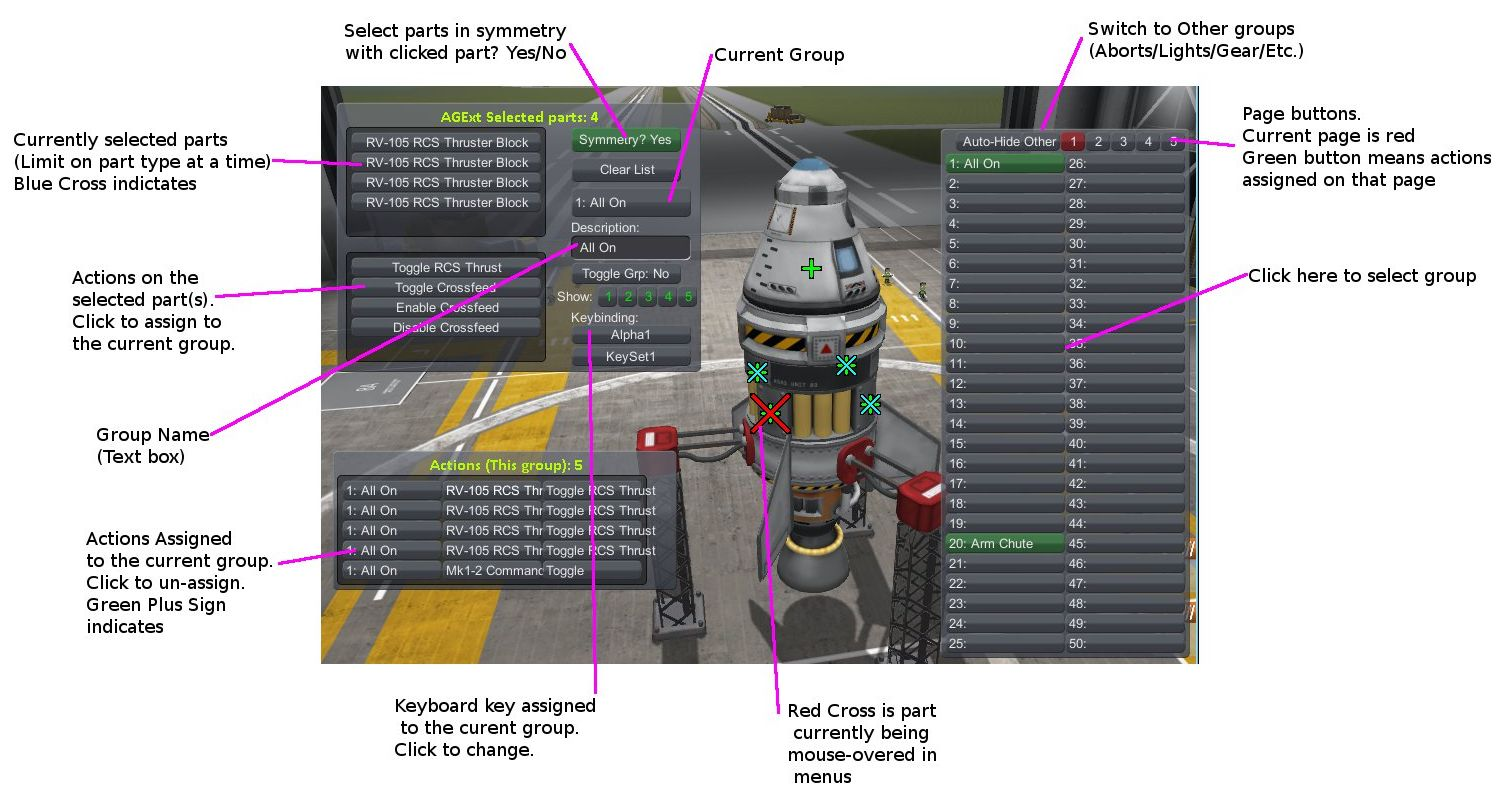
\includegraphics[width=6in]{AGExtQuickStart1.jpg}
\end{center}

\begin{center}
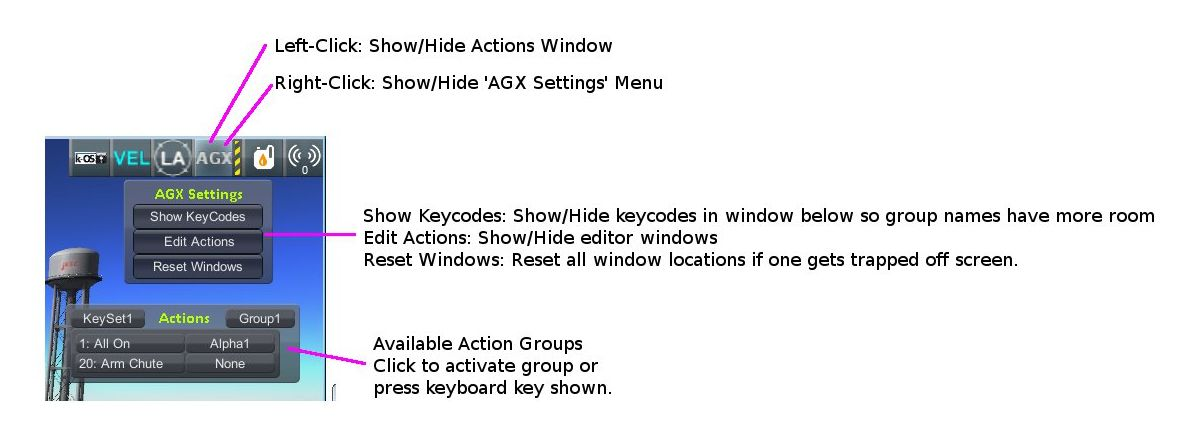
\includegraphics[width=6in]{AGExtQuickStart2.jpg}
\end{center}

Note that this mod only adds action groups 11 through 250, it does not change how action groups 1 through 10 behave in any way and groups 11 through 250 should behave the same way.

\subsection{Known limitations (Action groups 11 through 250 only):}

On a nearby vessel that is not your current focus, an action group with no actions assigned will always return a state of False and can not be set to a state of true via the ?AG15 on.? command. Assign the Script Trigger action as a work-around for this.

At this point, AG11 through AG250 do not officially support RemoteTech through kOS. (Support will happen once all three mods involved have updated to KSP version 1.0 and made any internal changes necessary.) All three mods can be installed at the same time without issue, just be aware there may be unexpected behaviour when using action groups 11 through 250 from a kOS script in terms of RemoteTech signal delay and connection state.

\subsection{Action state monitoring}

Note that the state of action groups is tracked on a per-action basis, rather then on a per-group basis. This results in the group state being handled differently.

The Script Trigger action found on the kOS computer module is not subject to the below considerations and is the recommended action to use when interacting with a running kOS script.
The state of actions are monitored on the part and updated automatically. A closed solar panel will return a state of false for all it?s actions. (Extend Panels, Retract Panels, Toggle Panels) When you extend the solar panel with either the Extend Panels or Toggle Panels action, all three actions will change to a state of True. Retract the panels and the state of all three actions will become False. Note that this state will update in any action group that contains that action, not just the action group that was activated.
This can result in an action group have actions in a mixed state where some actions are on and some are off. In this case querying the group state will result in a state of False. For the purposes of the group state being True or False, if all actions in the action group are true, the group state will return true. If any actions in the group are false,the group state with return False.
When an action triggers an animation, the state of the action will be uncertain until the animation finishes playing. Some parts will report True during the animation and some will report False. It depends on how the part creator set things up and not something AGX can control.
For clarity, visual feedback can be provided of the current state of an action group. When editing action groups, find the ?Toggle Grp.? button just below the text entry field for the group name in the main AGX window and enable it. (It is enabled/disabled for the current action group when you click the button.) Once you do this, the text displaying that group will change from gray to colored. Green: Group is activated (state True). Red: Group is deactivated (state False). Yellow: Group is in a mixed state, will return a state False when queried.
It is okay to activate an already activated group and deactivate a non-activated group. Actions in the group will still try to execute as normal. Exact behaviour of a specific action will depend on how the action?s creator set things up.

\subsection{Example code:}

Print to the terminal any time you activate action group 15. Use this to change variables within a running kOS script and the ?Script Trigger? action found on the kOS computer part:

\begin{lstlisting}[frame=single,language=XML]
AG15 on. // Activate action group 15.
print AG15. // Print action group 15's state to the terminal. (True/False)

on AG15 { //Prints "Action group 15 clicked!" to the console when AG15 is toggled, either via "AG15 on." or in-game with an assigned key.
  print "Action group 15 clicked!".
  preserve.
}
\end{lstlisting}

\subsection{Animation Delay:}

Using the above code on a stock solar panel?s Toggle Panels action, the player activates AG15, AG15?s state goes from false to true and the actions are triggered. AG15 False -> True and prints to the terminal.
On it?s next update pass (100ms to 250ms later), AGX checks AG15?s state and sees the solar panel is still deploying which means that AG15?s state is false and so sets it that way. AG15 True -> False and prints to the terminal.
A few seconds later, the solar panel finishes it?s deployment animation. On it?s next update pass AGX checks AG15?s state and sees the solar panel is now deployed which means that AG15?s state is now true and so sets it that way. AG15 False -> True and prints to the terminal a third time.
As a workaround, you need to add a cooldown:

\begin{lstlisting}[frame=single,language=XML]
declare cooldownTimeAG15 to 0.
on AG15 {
  if cooldownTimeAG15 + 10 < time:seconds {
    print "Solar Panel Toggled!".
    set cooldownTimeAG15 to time.
  }
  preserve.
}
\end{lstlisting}

Note the 10 in the second line, that is your cooldown time in seconds. Set this to a number of seconds that is longer then your animation time and the above code will limit whatever is inside the IF statement so it can only activate after 10 seconds have passed since the previous activation and will not try to activate a second time while the solar panel animation is still playing.
	\section{RemoteTech}%%%%% SECTION %%%%%
	RemoteTech is a modification for Squad?s ?Kerbal Space Program? (KSP) which overhauls the unmanned space program. It does this by requiring unmanned vessels have a connection to Kerbal Space Center (KSC) to be able to be controlled. This adds a new layer of difficulty that compensates for the lack of live crew members.
	\subsection{Interaction with kOS}
When you have RemoteTech installed you can only interact with the core?s terminal when you have a connection to KSC on any unmanned craft. Scripts launched when you still had a connection will continue to execute even if your unmanned craft loses connection to KSC. But you should note, that when there is no connection to KSC the archive volume is inaccessible. This will require you to plan ahead and copy necessary scripts for your mission to probe hard disk, if your kerbals and/or other scripts need to use them while not connected.

If you launch a manned craft while using RemoteTech, you are still able to input commands from the terminal even if you do not have a connection to the KSC. The archive will still be inaccessible without a connection to the KSC. Under the current implementation, there is no delay when accessing the archive with a local terminal. This implementation may change in the future to account for delays in reading and writing data over the connection.

It is possible to activate/deactivate RT antennas, as well as set their targets using kOS:

\begin{lstlisting}[frame=single,language=XML]
SET p TO SHIP:PARTSNAMED("mediumDishAntenna")[0].
SET m to p:GETMODULE("ModuleRTAntenna").
m:DOEVENT("activate").
m:SETFIELD("target", "mission-control").
// or
m:SETFIELD("target", mun).
m:SETFIELD("target", "minmus").
\end{lstlisting}

Acceptable values for ?target? are: ?no-target?, ?active-vessel?, ?mission-control?, a Body, a Vessel, or a string containing the name of a body or vessel.

Starting version 0.17 of kOS you can access structure RTAddon via ADDONS:RT.

structure RTAddon
Suffix	Type	Description
AVAILABLE	bool(readonly)	True if RT is installed and RT integration enabled.
DELAY(vessel)	double	Get shortest possible delay to given Vessel
KSCDELAY(vessel)	double	Get delay from KSC to given Vessel
HASCONNECTION(vessel)	bool	True if given Vessel has any connection
HASKSCCONNECTION(vessel)	bool	True if given Vessel has connection to KSC
HASLOCALCONTROL(vessel)	bool	True if given Vessel has local control
RTADDON:AVAILABLE
Type:	bool
Access:	Get only
True if RT is installed and RT integration enabled.

RTAddon:DELAY(vessel)
Parameters:	
vessel ? Vessel
Returns:	
(double) seconds

Returns shortest possible delay for vessel (Will be less than KSC delay if you have a local command post).

RTAddon:KSCDELAY(vessel)
Parameters:	
vessel ? Vessel
Returns:	
(double) seconds

Returns delay in seconds from KSC to vessel.

RTAddon:HASCONNECTION(vessel)
Parameters:	
vessel ? Vessel
Returns:	
bool

Returns True if vessel has any connection (including to local command posts).

RTAddon:HASKSCCONNECTION(vessel)
Parameters:	
vessel ? Vessel
Returns:	
bool

Returns True if vessel has connection to KSC.

RTAddon:HASLOCALCONTROL(vessel)
Parameters:	
vessel ? Vessel
Returns:	
bool

Returns True if vessel has local control (and thus not requiring a RemoteTech connection).
	\section{Kerbal Alarm Clock}%%%%% SECTION %%%%%
	The Kerbal Alarm Clock is a plugin that allows you to create reminder alarms at future periods to help you manage your flights and not warp past important times.

\begin{center}
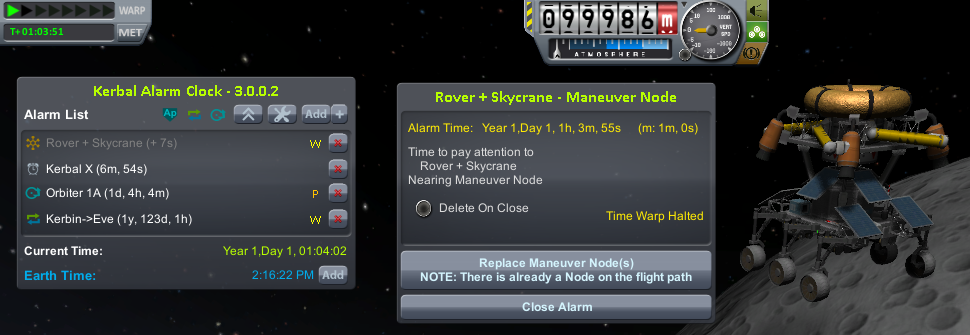
\includegraphics[width=6in]{KACForumPic.png}
\end{center}

Creator of the KAC provides API for integration with other mods. In KOS we provide limited access to KAC alarms via following structure and functions.

Access structure KACAddon via ADDONS:KAC.

structure KACAddon
Suffix	Type	Description
AVAILABLE	bool(readonly)	True if KAC is installed and KAC integration enabled.
ALARMS()	List	List all alarms
KACAddon:AVAILABLE
Type:	bool
Access:	Get only
True if KAC is installed and KAC integration enabled. Example of use:

\begin{lstlisting}[frame=single,language=XML]
if ADDONS:KAC:AVAILABLE
{
    //some KAC dependent code
}
\end{lstlisting}

KACAddon:ALARMS()
Returns:	List of KACAlarm objects
List all the alarms set up in Kerbal Alarm Clock. Example of use:

\begin{lstlisting}[frame=single,language=XML]
for i in ADDONS:KAC:ALARMS
{
        print i:NAME + " - " + i:REMAINING + " - " + i:TYPE+ " - " + i:ACTION.
}
\end{lstlisting}

structure KACAlarm
Suffix	Type	Description
ID	string (readonly)	Unique identifier
NAME	string	Name of the alarm
ACTION	string	What should the Alarm Clock do when the alarm fires
TYPE	string (readonly)	What type of Alarm is this - affects icon displayed and some calc options
NOTES	string	Long description of the alarm (optional)
REMAINING	scalar (s)	Time remaining until alarm is triggered
REPEAT	bool	Should the alarm be repeated once it fires
REPEATPERIOD	scalar (s)	How long after the alarm fires should the next alarm be set up
ORIGINBODY	string	Name of the body the vessel is departing from
TARGETBODY	string	Name of the body the vessel is arriving at
KACAlarm:ID
Type:	string
Access:	Get only
Unique identifier of the alarm.

KACAlarm:NAME
Type:	string
Access:	Get/Set
Name of the alarm. Displayed in main KAC window.

KACAlarm:ACTION
Type:	string
Access:	Get/Set
Should be one of the following

MessageOnly - Message Only-No Affect on warp
KillWarpOnly - Kill Warp Only-No Message
KillWarp - Kill Warp and Message
PauseGame - Pause Game and Message
If set incorrectly will log a warning in Debug log and revert to previous or default value.

KACAlarm:TYPE
Type:	string
Access:	Get only
Can only be set at Alarm creation. Could be one of the following as per API

Raw (default)
Maneuver
ManeuverAuto
Apoapsis
Periapsis
AscendingNode
DescendingNode
LaunchRendevous
Closest
SOIChange
SOIChangeAuto
Transfer
TransferModelled
Distance
Crew
EarthTime
Warning: Unless you are 100\% certain you know what you?re doing, create only ?Raw? AlarmTypes to avoid unnecessary complications.

KACAlarm:NOTES
Type:	string
Access:	Get/Set
Long description of the alarm. Can be seen when alarm pops or by double-clicking alarm in UI.

Warning: This field may be reserved in the future version of KAC-KOS integration for automated script execution upon triggering of the alarm.

KACAlarm:REMAINING
Type:	double
Access:	Get only
Time remaining until alarm is triggered.

KACAlarm:REPEAT
Type:	bool
Access:	Get/Set
Should the alarm be repeated once it fires.

KACAlarm:REPEATPERIOD
Type:	double
Access:	Get/Set
How long after the alarm fires should the next alarm be set up.

KACAlarm:ORIGINBODY
Type:	string
Access:	Get/Set
Name of the body the vessel is departing from.

KACAlarm:TARGETBODY
Type:	string
Access:	Get/Set
Name of the body the vessel is arriving to.

Available Functions
Function	Description
ADDALARM(AlarmType, UT, Name, Notes)	Create new alarm of AlarmType at UT
LISTALARMS(alarmType)	List alarms with type alarmType.
DELETEALARM(alarmID)	Delete alarm with ID = alarmID
ADDALARM(AlarmType, UT, Name, Notes)
Creates alarm of type KACAlarm:ALARMTYPE at UT with Name and Notes attributes set. Attaches alarm to current CPU Vessel. Returns KACAlarm object if creation was successful and empty string otherwise:

\begin{lstlisting}[frame=single,language=XML]
set na to addAlarm("Raw",time:seconds+300, "Test", "Notes").
print na:NAME. //prints 'Test'
set na:NOTES to "New Description".
print na:NOTES. //prints 'New Description'
\end{lstlisting}

LISTALARMS(alarmType)
If alarmType equals ?All?, returns List of all KACAlarm objects attached to current vessel or have no vessel attached. Otherwise returns List of all KACAlarm objects with KACAlarm:TYPE equeal to alarmType and attached to current vessel or have no vessel attached.:

\begin{lstlisting}[frame=single,language=XML]
set al to listAlarms("All").
for i in al
{
    print i:ID + " - " + i:name.
}
\end{lstlisting}

DELETEALARM(alarmID)
Deletes alarm with ID equal to alarmID. Returns True if successful, false otherwise:

\begin{lstlisting}[frame=single,language=XML]
set na to addAlarm("Raw",time:seconds+300, "Test", "Notes").
if (DELETEALARM(na:ID))
{
    print "Alarm Deleted".
}
\end{lstlisting}
	\section{Infernal Robotics}%%%%% SECTION %%%%%
	Infernal Robotics introduces robotics parts to the game, letting you create moving or spinning contraptions that just aren?t possible under stock KSP.
	
\begin{center}

\includegraphics[width=6in]{O94LBvF.png}
\end{center}

Starting version 0.20 of the Infernal Robotics, mod creators introduced API to for easier access to robotic features.

Access structure IRAddon via ADDONS:IR.

structure IRAddon
Suffix	Type	Description
AVAILABLE	bool(readonly)	Returns True if mod Infernal Robotics is installed, available to KOS and applicable to current craft.
GROUPS	List (readonly)	Lists all Servo Groups for current focused vessel
ALLSERVOS	List (readonly)	Lists all Servos for current focused vessel
IRAddon:AVAILABLE
Type:	bool
Access:	Get only
Returns True if mod Infernal Robotics is installed, available to KOS and applicable to current craft. Example of use:

\begin{lstlisting}[frame=single,language=XML]
if ADDONS:IR:AVAILABLE
{
    //some IR dependent code
}
\end{lstlisting}

IRAddon:GROUPS
Type:	List of IRControlGroup objects
Access:	Get only
Lists all Servo Groups for current focused vessel. Example of use:

\begin{lstlisting}[frame=single,language=XML]
for g in ADDONS:IR:GROUPS
{
    Print g:NAME + " contains " + g:SERVOS:LENGTH + " servos".
}
\end{lstlisting}

IRAddon:ALLSERVOS
Type:	List of IRServo objects
Access:	Get only
Lists all Servos for current focused vessel. Example of use:

\begin{lstlisting}[frame=single,language=XML]
for s in ADDONS:IR:ALLSERVOS
{
    print "Name: " + s:NAME + ", position: " + s:POSITION.
}
\end{lstlisting}

structure IRControlGroup
Suffix	Type	Description
NAME	string	Name of the Control Group
SPEED	float	Speed multiplier set in the IR UI
EXPANDED	bool	True if Group is expanded in IR UI
FORWARDKEY	string	Key assigned to forward movement
REVERSEKEY	string	Key assigned to reverse movement
SERVOS	List (readonly)	List of servos in the group
MOVERIGHT()	void	Commands servos in the group to move in positive direction
MOVELEFT()	void	Commands servos in the group to move in negative direction
MOVECENTER()	void	Commands servos in the group to move to default position
MOVENEXTPRESET()	void	Commands servos in the group to move to next preset
MOVEPREVPRESET()	void	Commands servos in the group to move to previous preset
STOP()	void	Commands servos in the group to stop
IRControlGroup:NAME
Type:	string
Access:	Get/Set
Name of the Control Group (cannot be empty).

IRControlGroup:SPEED
Type:	float
Access:	Get/Set
Speed multiplier as set in the IR user interface. Avoid setting it to 0.

IRControlGroup:EXPANDED
Type:	bool
Access:	Get/Set
True if Group is expanded in IR UI

IRControlGroup:FORWARDKEY
Type:	string
Access:	Get/Set
Key assigned to forward movement. Can be empty.

IRControlGroup:REVERSEKEY
Type:	string
Access:	Get/Set
Key assigned to reverse movement. Can be empty.

IRControlGroup:SERVOS
Type:	List of IRServo objects
Access:	Get only
Lists Servos in the Group. Example of use:

\begin{lstlisting}[frame=single,language=XML]
for g in ADDONS:IR:GROUPS
{
    Print g:NAME + " contains " + g:SERVOS:LENGTH + " servos:".
    for s in g:servos
    {
        print "    " + s:NAME + ", position: " + s:POSITION.
    }
}
\end{lstlisting}

IRControlGroup:MOVERIGHT()
Returns:	void
Commands servos in the group to move in positive direction.

IRControlGroup:MOVELEFT()
Returns:	void
Commands servos in the group to move in negative direction.

IRControlGroup:MOVECENTER()
Returns:	void
Commands servos in the group to move to default position.

IRControlGroup:MOVENEXTPRESET()
Returns:	void
Commands servos in the group to move to next preset

IRControlGroup:MOVEPREVPRESET()
Returns:	void
Commands servos in the group to move to previous preset

IRControlGroup:STOP()
Returns:	void
Commands servos in the group to stop

structure IRServo
Suffix	Type	Description
NAME	string	Name of the Servo
UID	int	Unique ID of the servo part (part.flightID).
HIGHLIGHT	bool (set-only)	Set Hightlight status of the part.
POSITION	float (readonly)	Current position of the servo.
MINCFGPOSITION	float (readonly)	Minimum position for servo as defined by part creator in part.cfg
MAXCFGPOSITION	float (readonly)	Maximum position for servo as defined by part creator in part.cfg
MINPOSITION	float	Minimum position for servo, from tweakable.
MAXPOSITION	float	Maximum position for servo, from tweakable.
CONFIGSPEED	float (readonly)	Servo movement speed as defined by part creator in part.cfg
SPEED	float	Servo speed multiplier, from tweakable.
CURRENTSPEED	float (readonly)	Current Servo speed.
ACCELERATION	float	Servo acceleration multiplier, from tweakable.
ISMOVING	bool (readonly)	True if Servo is moving
ISFREEMOVING	bool (readonly)	True if Servo is uncontrollable (ex. docking washer)
LOCKED	bool	Servo?s locked status, set true to lock servo.
INVERTED	bool	Servo?s inverted status, set true to invert servo?s axis.
MOVERIGHT()	void	Commands servo to move in positive direction
MOVELEFT()	void	Commands servo to move in negative direction
MOVECENTER()	void	Commands servo to move to default position
MOVENEXTPRESET()	void	Commands servo to move to next preset
MOVEPREVPRESET()	void	Commands servo to move to previous preset
STOP()	void	Commands servo to stop
MOVETO(position, speedMult)	void	Commands servo to move to position with speedMult multiplier
IRServo:NAME
Type:	string
Access:	Get/Set
Name of the Control Group (cannot be empty).

IRServo:UID
Type:	int
Access:	Get
Unique ID of the servo part (part.flightID).

IRServo:HIGHLIGHT
Type:	bool
Access:	Set
Set Hightlight status of the part.

IRServo:POSITION
Type:	float
Access:	Get
Current position of the servo.

IRServo:MINCFGPOSITION
Type:	float
Access:	Get
Minimum position for servo as defined by part creator in part.cfg

IRServo:MAXCFGPOSITION
Type:	float
Access:	Get
Maximum position for servo as defined by part creator in part.cfg

IRServo:MINPOSITION
Type:	float
Access:	Get/Set
Minimum position for servo, from tweakable.

IRServo:MAXPOSITION
Type:	float
Access:	Get/Set
Maximum position for servo, from tweakable.

IRServo:CONFIGSPEED
Type:	float
Access:	Get
Servo movement speed as defined by part creator in part.cfg

IRServo:SPEED
Type:	float
Access:	Get/Set
Servo speed multiplier, from tweakable.

IRServo:CURRENTSPEED
Type:	float
Access:	Get
Current Servo speed.

IRServo:ACCELERATION
Type:	float
Access:	Get/Set
Servo acceleration multiplier, from tweakable.

IRServo:ISMOVING
Type:	bool
Access:	Get
True if Servo is moving

IRServo:ISFREEMOVING
Type:	bool
Access:	Get
True if Servo is uncontrollable (ex. docking washer)

IRServo:LOCKED
Type:	bool
Access:	Get/Set
Servo?s locked status, set true to lock servo.

IRServo:INVERTED
Type:	bool
Access:	Get/Set
Servo?s inverted status, set true to invert servo?s axis.

IRServo:MOVERIGHT()
Returns:	void
Commands servo to move in positive direction

IRServo:MOVELEFT()
Returns:	void
Commands servo to move in negative direction

IRServo:MOVECENTER()
Returns:	void
Commands servo to move to default position

IRServo:MOVENEXTPRESET()
Returns:	void
Commands servo to move to next preset

IRServo:MOVEPREVPRESET()
Returns:	void
Commands servo to move to previous preset

IRServo:STOP()
Returns:	void
Commands servo to stop

IRServo:MOVETO(position, speedMult)
Parameters:	
position ? (float) Position to move to
speedMult ? (float) Speed multiplier
Returns:	
void

Commands servo to move to position with speedMult multiplier.

Example code:

\begin{lstlisting}[frame=single,language=XML]
print "IR Iavailable: " + ADDONS:IR:AVAILABLE.

Print "Groups:".

for g in ADDONS:IR:GROUPS
{
    Print g:NAME + " contains " + g:SERVOS:LENGTH + " servos:".
    for s in g:servos
    {
        print "    " + s:NAME + ", position: " + s:POSITION.
        if (g:NAME = "Hinges" and s:POSITION = 0)
        {
            s:MOVETO(30, 2).
        }
        else if (g:NAME = "Hinges" and s:POSITION > 0)
        {
            s:MOVETO(0, 1).
        }
    }
}
\end{lstlisting}